\documentclass[11pt,a4paper]{article}

% Packages
\usepackage[utf8]{inputenc}
\usepackage[english]{babel}
\usepackage{graphicx}
\usepackage{geometry}
\usepackage{hyperref}
\usepackage{longtable}
\usepackage{booktabs}
\usepackage{array}
\usepackage{enumitem}
\usepackage{titlesec}
\usepackage{listings}
\usepackage{xcolor}
\usepackage{float}
\usepackage{ragged2e}
\usepackage{microtype}

% Page geometry
\geometry{a4paper, margin=2.5cm}

% Hyperref setup
\hypersetup{
    colorlinks=true,
    linkcolor=blue,
    filecolor=magenta,      
    urlcolor=cyan,
    pdftitle={Smart Audiobook Player Project Report},
    pdfauthor={John Nguyen, Khaled Rami Omar, Jahye Ali},
}

% Title formatting
\titleformat{\section}{\Large\bfseries}{\thesection}{1em}{}
\titleformat{\subsection}{\large\bfseries}{\thesubsection}{1em}{}
\titleformat{\subsubsection}{\normalsize\bfseries}{\thesubsubsection}{1em}{}

% Code listing setup
\lstset{
    basicstyle=\ttfamily\small,
    breaklines=true,
    frame=single,
    backgroundcolor=\color{gray!10}
}

\begin{document}

% Title Page
\begin{titlepage}
    \centering
    \vspace*{2cm}
    
    {\Huge\bfseries Smart Audiobook Player\par}
    \vspace{0.5cm}
    {\Large Project Report\par}
    \vspace{2cm}
    
    {\large
    \textbf{Course:} Mobile Application Development\par
    \vspace{0.5cm}
    \textbf{Report Type:} Final Project Rapport\par
    \vspace{1cm}
    
    \textbf{Group Members:}\par
    \vspace{0.3cm}
    John Nguyen (202209849)\par
    Khaled Rami Omar (202307853)\par
    Jahye Ali (202309135)\par
    \vspace{1cm}
    
    \textbf{Delivery Date:} 25 March 2026\par
    }
    
    \vfill
\end{titlepage}

% Table of Contents
\tableofcontents
\clearpage

% Main Content
\section{App Vision}

Smart Audiobook Player is a premium mobile audiobook app focused on smooth long-form listening, especially for M4B/M4A files.

The app solves common audiobook pain points: poor chapter support, weak resume accuracy, and inconsistent playback across sessions/devices. It offers secure user accounts, cloud-synced progress, chapter-aware playback, and a minimalist high-contrast interface designed for distraction-free listening.

\section{Features and Requirements Specification}

This section maps the requested project requirements to the implemented Android solution.

\subsection{Implemented Feature Overview}

Smart Audiobook Player is implemented as a Kotlin Android app using Jetpack Compose and an MVVM-style architecture. Core playback is built on Media3, where a \texttt{MediaSessionService} (\texttt{PlaybackService}) handles background playback and system integrations. UI and service are connected through a \texttt{MediaController} wrapper (\texttt{AudiobookPlayer}) and Compose state flows.

\textbf{Important:} All audiobook files (M4B/M4A format) are stored locally on the device's filesystem. The app scans device storage directories (e.g., \texttt{/storage/emulated/0/Audiobooks/}) to discover available audiobooks. Room database stores only metadata (title, author, file path, cover art path) and playback progress---not the audio files themselves. ExoPlayer streams audio directly from local file URIs during playback.

The app includes the requested core screens:
\begin{itemize}[noitemsep]
    \item Library screen with search, continue listening, folder selection, and grid browsing
    \item Player screen with play/pause, seek, chapter support, speed control, and sleep timer
    \item Book details screen with metadata, chapter list, and progress-focused actions
    \item Profile and settings flows for notification preferences and app behavior
\end{itemize}

It also includes advanced features from the synopsis:
\begin{itemize}[noitemsep]
    \item Firebase integration (\texttt{AuthRepository}, Firestore-based progress/notification services)
    \item Biometric lock entry flow (\texttt{LibraryLockedScreen} and \texttt{BiometricPrompt} in \texttt{MainActivity})
    \item Metadata enrichment through manual HTTP API calls (OpenLibrary via Retrofit/OkHttp)
    \item Notification services (local scheduled reminders and FCM handling)
\end{itemize}

\subsection{Requirements Traceability Matrix}

{\small
\begin{longtable}{|p{0.8cm}|>{\RaggedRight}p{4.5cm}|>{\RaggedRight}p{2.5cm}|>{\RaggedRight}p{5.5cm}|}
\hline
\textbf{ID} & \textbf{Requirement} & \textbf{Status} & \textbf{Notes / Evidence} \\ \hline
\endfirsthead
\hline
\textbf{ID} & \textbf{Requirement} & \textbf{Status} & \textbf{Notes / Evidence} \\ \hline
\endhead
R1 & M4B/M4A audiobook playback & Implemented & Media3 \texttt{ExoPlayer} + \texttt{Playback-} \texttt{Service} (\texttt{MediaSessionService}) \\ \hline
R2 & Background playback with system integration & Implemented & Media session service, custom skip commands, notification integration \\ \hline
R3 & Library browsing and search & Implemented & \texttt{LibraryViewModel} + \texttt{LibraryScreen} reactive filtering \\ \hline
R4 & Chapter-aware playback & Implemented & \texttt{ChapterParser}, chapter-relative seek/progress, chapter bottom sheet \\ \hline
R5 & Resume from saved position & Implemented & Position persisted and restored in \texttt{PlayerViewModel} + repositories \\ \hline
R6 & Playback speed control (0.5x to 2.0x) & Implemented & Speed options and persistence in preferences \\ \hline
R7 & Sleep timer & Implemented & Timed mode + end-of-chapter mode in \texttt{PlayerViewModel} \\ \hline
R8 & Firestore cross-device progress sync & Partially integrated & \texttt{ProgressSync-} \texttt{Repository} exists with full API, but not fully wired into main playback flow \\ \hline
R9 & Firebase authentication for user account flows & Partially integrated & Auth repository is present; dedicated sign-in/sign-up UI flow is not fully wired in navigation \\ \hline
R10 & Biometric library lock & Partially integrated & Lock UI and prompt exist; device fallback currently bypasses lock for demo path \\ \hline
R11 & Notification workflows (daily, streak, milestones) & Implemented (with caveats) & Scheduler + trigger helper + FCM service; multiple silent-failure catches remain \\ \hline
R12 & Metadata enrichment via external HTTP API & Implemented & OpenLibrary API client and repository integration \\ \hline
\end{longtable}
}

\subsection{Non-Functional Requirements and Engineering Choices}

\begin{itemize}[noitemsep]
    \item \textbf{Performance and UX responsiveness:} Playback state and progress are exposed as \texttt{StateFlow}, which keeps Compose UI reactive and avoids heavy polling in the UI layer.
    \item \textbf{State persistence:} Local Room and DataStore persistence support app restarts and consistent resume behavior.
    \item \textbf{Reliability:} Error handling exists in most repositories, but several notification and remote paths still swallow errors, reducing observability.
    \item \textbf{Maintainability:} Manual DI (\texttt{AppContainer}) keeps dependencies explicit and project setup simple.
    \item \textbf{Compatibility:} Minimum SDK 26 and modern target/compile SDK 35 configuration.
\end{itemize}

\section{User Stories (Selected Non-Trivial)}

The following stories were selected because they combine multiple subsystems (UI, media service, persistence, and cloud/backend features).

\subsection{User Story 1 - Chapter-aware Listening}

\textbf{Story:} As a listener, I want to navigate by chapter so I can jump directly to meaningful parts of long audiobooks.

\textbf{Acceptance focus:}
\begin{itemize}[noitemsep]
    \item Chapters are extracted from M4B metadata
    \item The player can seek to chapter start
    \item Current chapter is detected from playback position
    \item Chapter-relative progress is shown
\end{itemize}

\textbf{Implementation status:} Implemented. \texttt{PlayerViewModel} calculates current chapter and chapter progress continuously. \texttt{PlayerScreen} exposes a chapter sheet and chapter-aware seek behavior.

\subsection{User Story 2 - Exact Resume After Interruption}

\textbf{Story:} As a listener, I want to resume exactly where I stopped so I do not lose context in long sessions.

\textbf{Acceptance focus:}
\begin{itemize}[noitemsep]
    \item Position is saved during/after playback
    \item Re-opening a book resumes from saved position
    \item Resume works across screen changes and app restarts
\end{itemize}

\textbf{Implementation status:} Implemented. Progress updates are persisted frequently (debounced updates in player view model), and playback resumes using saved positions.

\subsection{User Story 3 - Cross-device Continuity}

\textbf{Story:} As an authenticated user, I want my progress in the cloud so I can continue on another device.

\textbf{Acceptance focus:}
\begin{itemize}[noitemsep]
    \item Progress can be pushed to Firestore
    \item Cloud progress can be pulled and merged locally
    \item Real-time observation is possible
\end{itemize}

\textbf{Implementation status:} Partially integrated. \texttt{ProgressSyncRepository} contains save/pull/observe/sync APIs and Firestore schema, but call-sites are not fully connected through the main playback lifecycle.

\subsection{User Story 4 - Secure Access to Private Library}

\textbf{Story:} As a user, I want biometric gatekeeping so unauthorized users cannot open my audiobook library.

\textbf{Acceptance focus:}
\begin{itemize}[noitemsep]
    \item Lock screen appears when enabled
    \item Unlock requires successful biometric authentication
\end{itemize}

\textbf{Implementation status:} Partially integrated. Biometric prompt and lock screen exist, but the current fallback path allows bypass when strong biometrics are unavailable. Also, no clear in-app toggle currently drives \texttt{setRememberBiometric(...)}.

\subsection{User Story 5 - Smart Engagement Notifications}

\textbf{Story:} As a listener, I want reminders and milestone notifications so I can maintain consistency and motivation.

\textbf{Acceptance focus:}
\begin{itemize}[noitemsep]
    \item Daily reminders can be scheduled
    \item Streak and milestone events can trigger notifications
    \item Notification preferences are configurable
\end{itemize}

\textbf{Implementation status:} Implemented with operational caveats. Daily/streak/milestone systems are implemented in scheduler and trigger helpers, with settings controls. Several catch blocks silently ignore errors, which may hide delivery issues.

\section{Diagrams}

\subsection{UI Diagrams / Sketches}

Primary UI sketches and emulator captures are available in project assets:

\begin{figure}[H]
\centering
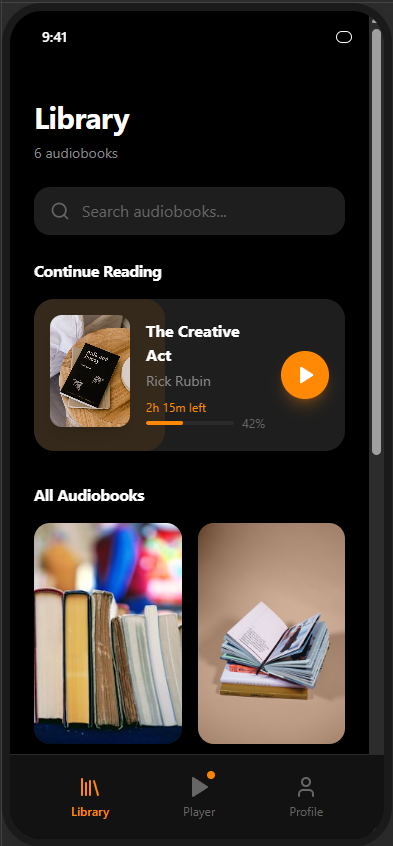
\includegraphics[width=0.4\textwidth]{../Figma pictures/HomeScreen - Library.png}
\caption{Library Screen}
\end{figure}

\begin{figure}[H]
\centering
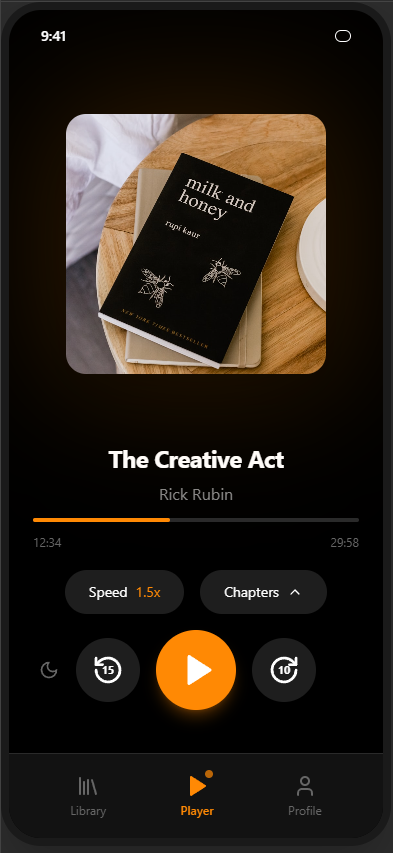
\includegraphics[width=0.4\textwidth]{../Figma pictures/Player Page.png}
\caption{Player Screen}
\end{figure}

\begin{figure}[H]
\centering
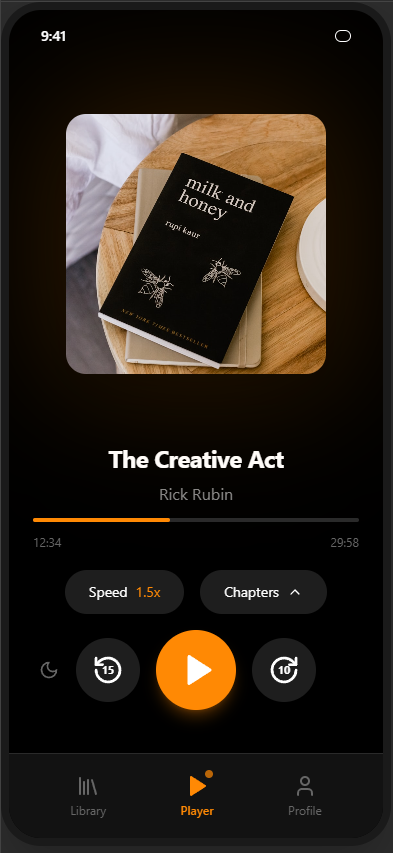
\includegraphics[width=0.4\textwidth]{../Figma pictures/Profile Page.png}
\caption{Profile Screen}
\end{figure}

\begin{figure}[H]
\centering
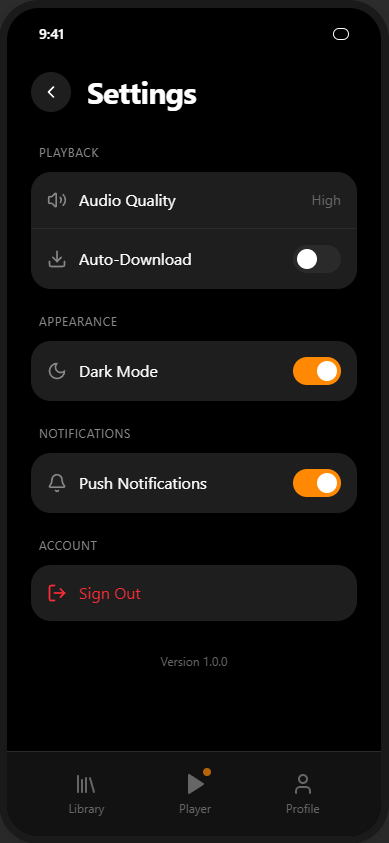
\includegraphics[width=0.4\textwidth]{../Figma pictures/Settings Page.png}
\caption{Settings Screen}
\end{figure}

\subsection{UI Flow Diagram}

\begin{figure}[H]
\centering
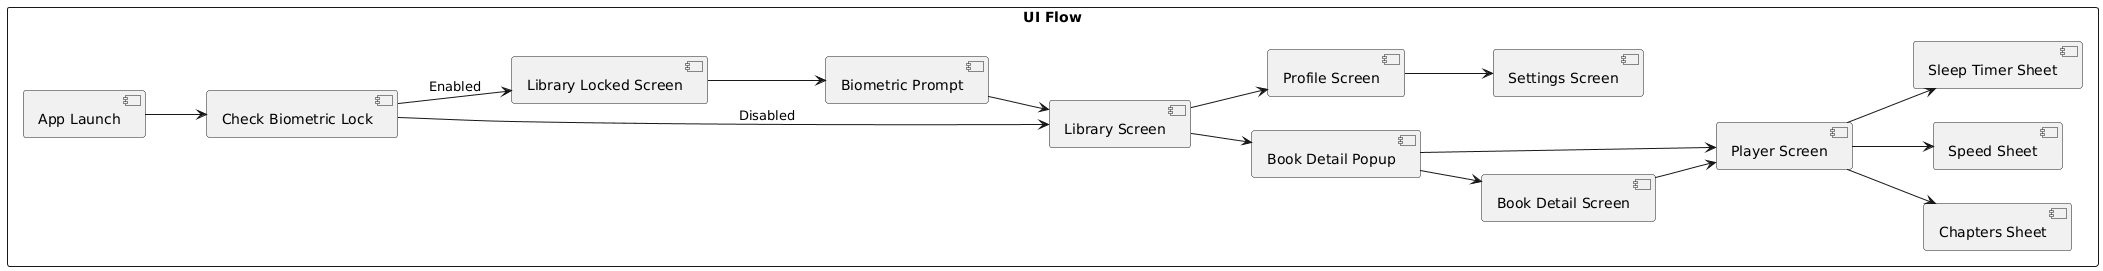
\includegraphics[width=0.9\textwidth]{./diagrams/exports/ui_flow.png}
\caption{UI Flow Diagram}
\end{figure}

The UI flow begins with app launch and biometric authentication check (if enabled). Users navigate from the library to book details and player screens, with access to settings and profile screens. The player screen provides access to chapters, playback speed, and sleep timer controls.

\subsection{Component Diagram}

\begin{figure}[H]
\centering

\includegraphics[width=0.95\textwidth]{./diagrams/exports/component_diagram.png}
\caption{Component Architecture Diagram}
\end{figure}

The architecture follows clean MVVM patterns with clear separation between UI layer (Compose screens), ViewModel layer, Data/Domain layer (repositories), Playback layer (Media3 components), local storage (Room/DataStore for metadata and preferences), and external services (Firebase, OpenLibrary API). 

\textbf{Device Storage Integration:} The \texttt{AudiobookScanner} component scans the device filesystem to discover M4B/M4A audiobook files stored locally. \texttt{ExoPlayer} streams audio directly from these local file paths during playback. Only metadata and progress are persisted in Room database---the actual audio files remain in device storage and are never copied or moved.

\subsection{Use Case Diagram}

\begin{figure}[H]
\centering
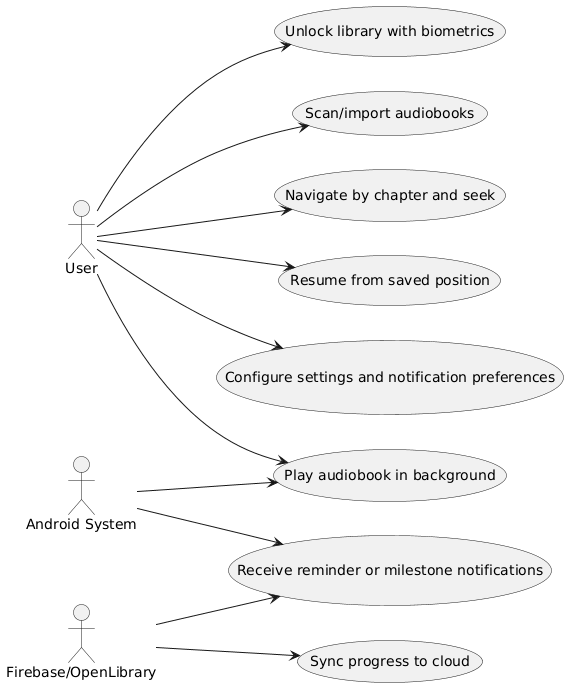
\includegraphics[width=0.9\textwidth]{./diagrams/exports/use_case_diagram.png}
\caption{Use Case Diagram}
\end{figure}

Key use cases include biometric authentication, audiobook scanning/import, background playback, chapter navigation, position resume, cloud progress sync, notification handling, and settings configuration. These involve interactions between the user, Android system, and cloud services.

\subsection{Sequence Diagram - Audio Playback Flow}

\begin{figure}[H]
\centering
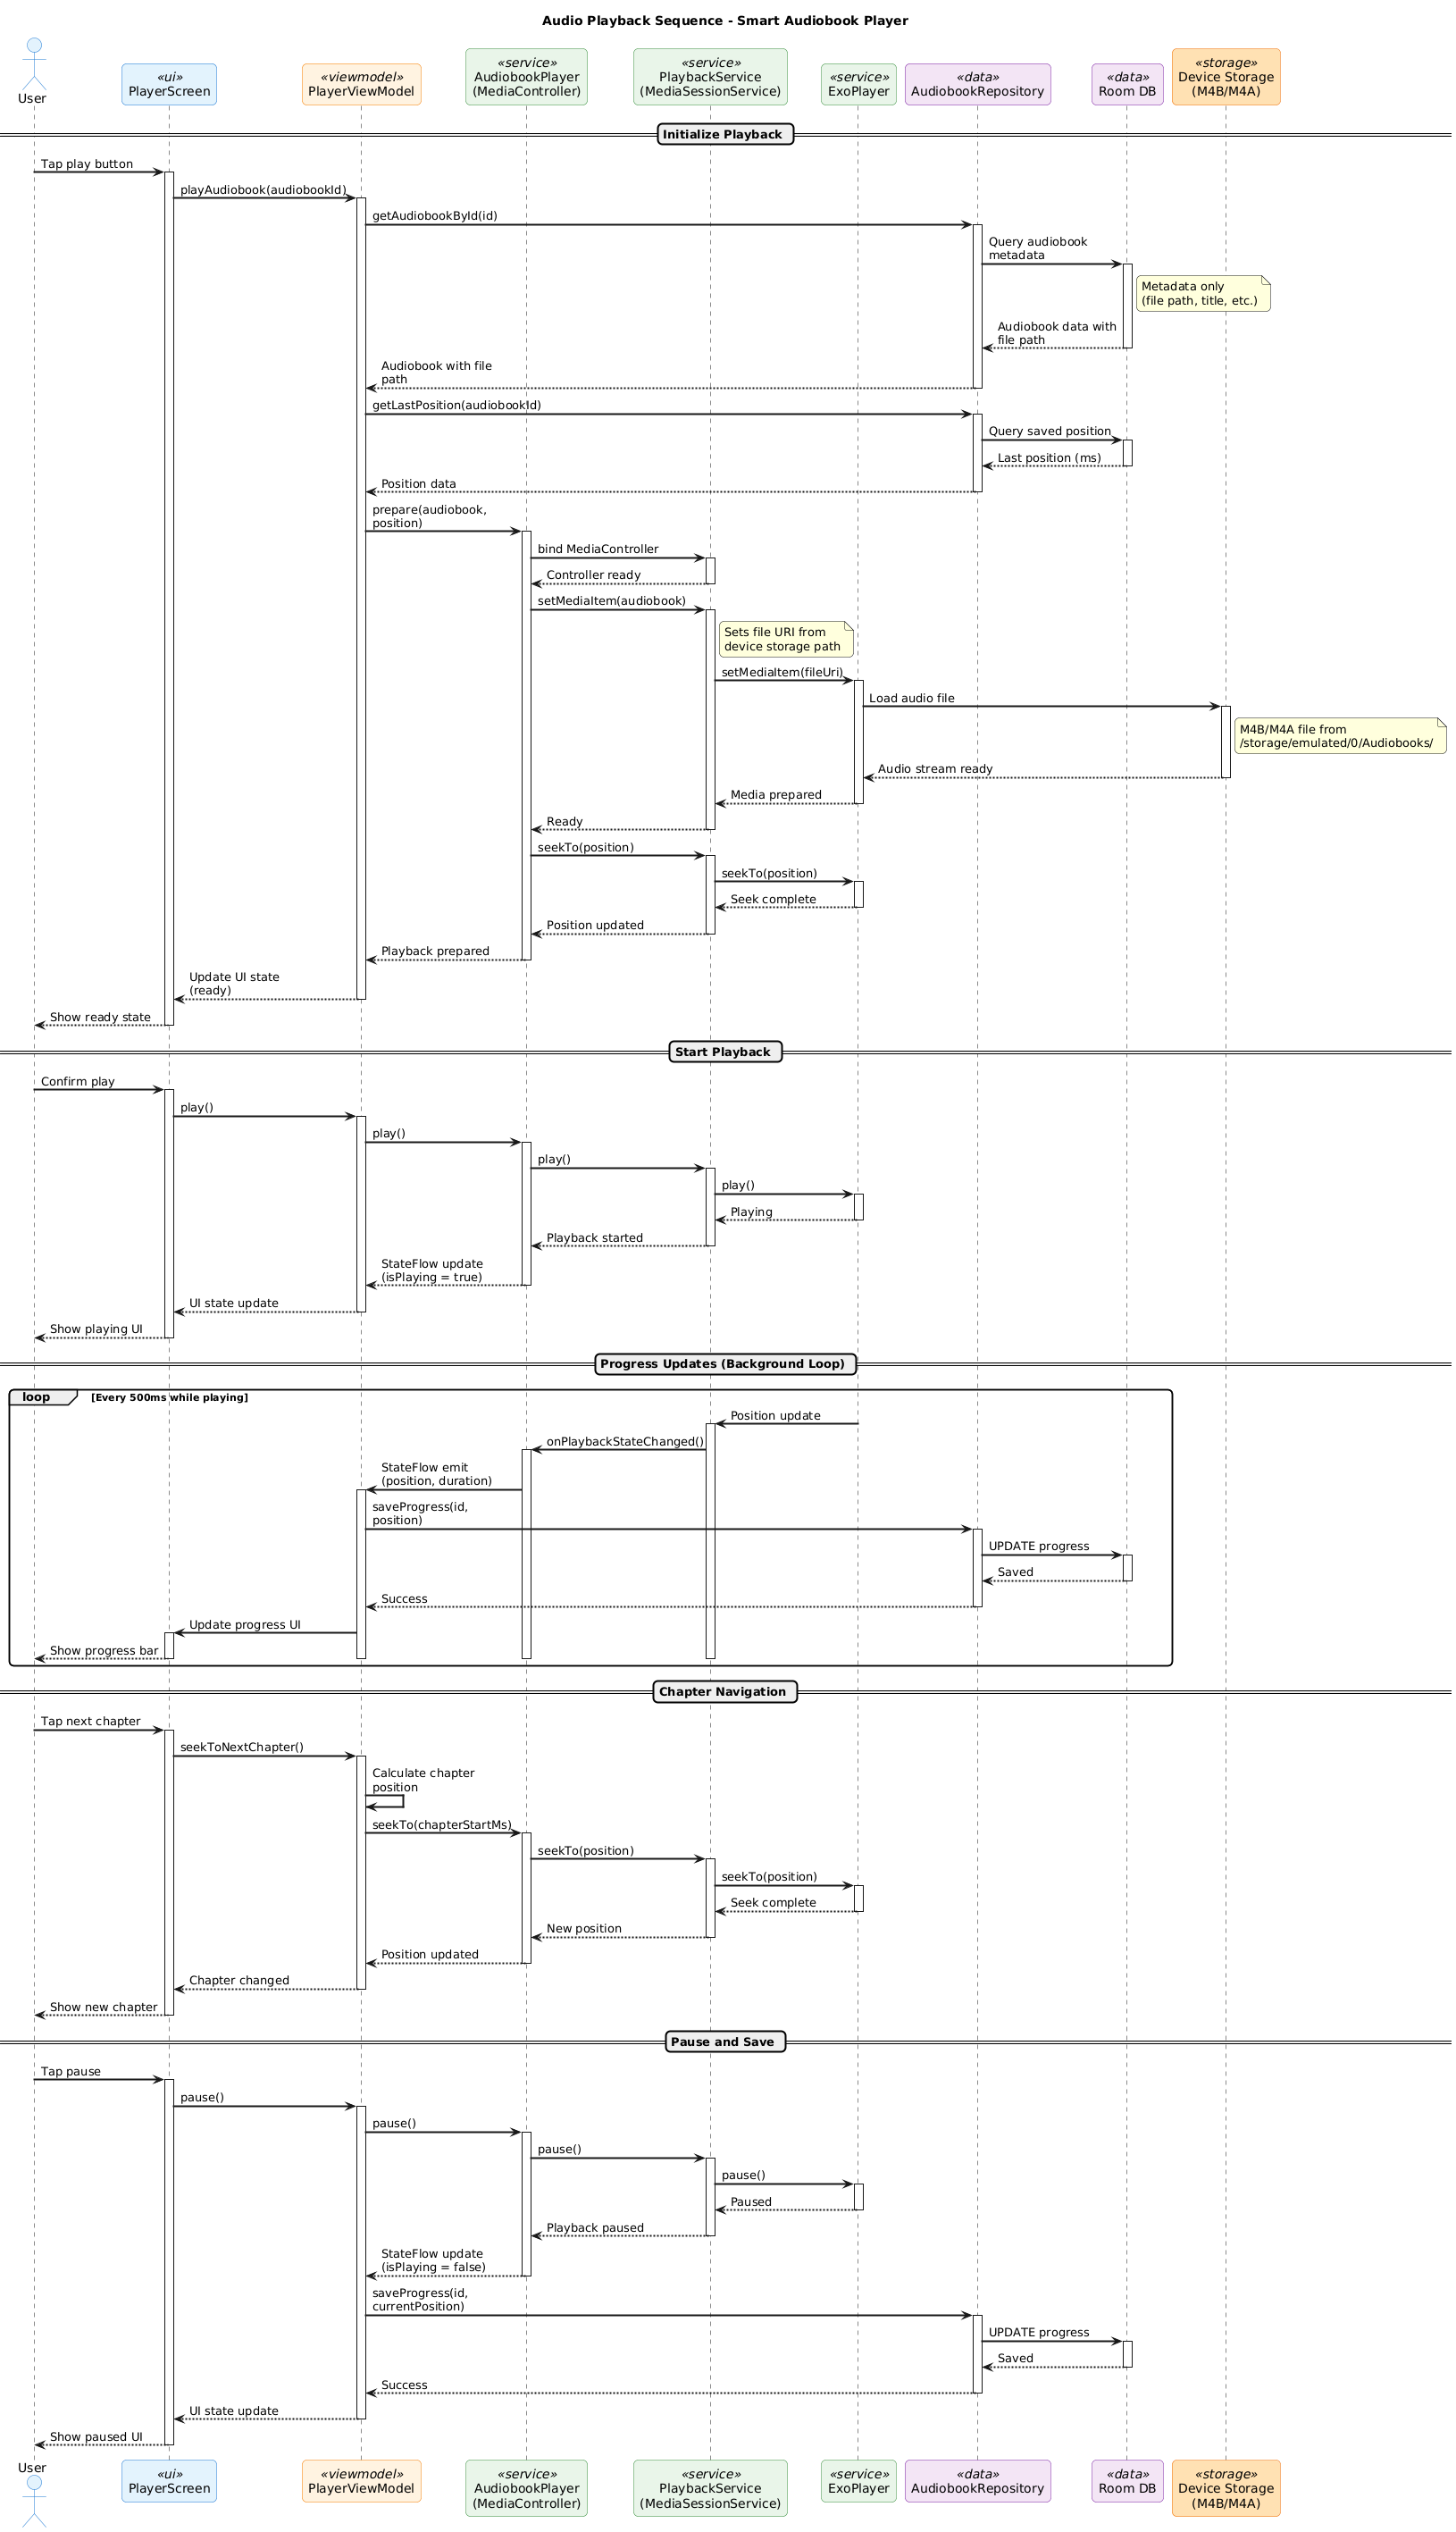
\includegraphics[width=\textwidth]{./diagrams/exports/sequence_playback.png}
\caption{Audio Playback Sequence Diagram}
\end{figure}

The sequence diagram illustrates the complete audio playback lifecycle, capturing five key interaction phases:

\begin{enumerate}[noitemsep]
    \item \textbf{Initialization:} User taps play, triggering a chain that loads audiobook metadata (including local file path) and last saved position from Room database. The \texttt{PlayerViewModel} coordinates retrieval through \texttt{AudiobookRepository}. Note: Room stores only metadata; the actual M4B/M4A file remains in device storage.
    
    \item \textbf{Media preparation:} The \texttt{AudiobookPlayer} (MediaController facade) binds to \texttt{PlaybackService} and configures the underlying \texttt{ExoPlayer} with the media item. ExoPlayer loads the audio file directly from the device filesystem using the local file URI (e.g., \texttt{file:///storage/emulated/0/Audiobooks/book.m4b}).
    
    \item \textbf{Playback control:} User confirmation triggers play command down through the layers to ExoPlayer, which begins streaming audio from the local file. State updates flow back up through StateFlow emissions, keeping UI reactive.
    
    \item \textbf{Progress tracking:} A background loop runs every 500ms during playback, persisting current position to Room DB. This enables accurate resume and progress continuity without affecting the source audio file.
    
    \item \textbf{Chapter navigation:} User-initiated chapter jumps calculate target position in \texttt{PlayerViewModel}, issue seek commands to the playback service, and update UI with new chapter context. All chapter metadata is extracted from the M4B file itself during initial scanning.
\end{enumerate}

This design demonstrates clear separation of concerns: UI layer handles user interaction, ViewModel manages state and business logic, service layer handles media playback lifecycle and streams from device storage, and repository layer abstracts metadata persistence. The unidirectional data flow (actions down, state up) follows Android best practices for predictable state management.

\section{Conclusion}

Smart Audiobook Player delivers a strong end-to-end Android audiobook experience that aligns with the course goals and the original synopsis direction.The project demonstrates practical use of modern Android architecture and media APIs, especially through the Media3 \texttt{MediaSessionService} approach, chapter-aware playback logic, and a Compose-first UI implementation.

From a technical perspective, the main success is the playback architecture: decoupling UI from media service, preserving playback continuity, and supporting audiobook-specific controls such as 15s/30s skip, chapter navigation, speed control, and sleep timer. The implementation also shows good persistence strategy through Room and DataStore, enabling reliable local resume behavior.

Firebase and notification capabilities are present and substantial, and the project includes advanced ideas such as engagement tracking and milestone-based reminders. In addition, metadata and chapter extraction challenges were investigated deeply, and chapter compatibility improvements were documented, including fallback parsing strategies and generation-side chapter metadata fixes.

The most important insights gained during development were:
\begin{itemize}[noitemsep]
    \item Media containers are inconsistent in chapter metadata encoding, so robust fallback parsing is essential
    \item Long-form audio apps need frequent but controlled persistence updates to balance accuracy and performance
    \item Cloud sync is not only a repository problem; it must be carefully wired into lifecycle and conflict-resolution flows to become truly production-ready
    \item UX security features (such as biometrics) require complete settings integration, not just prompt-level implementation
\end{itemize}

Overall, the project is technically mature in core playback and UI/UX foundations and provides a solid baseline for future production hardening.

\section{Known Bugs and Issues}

{\footnotesize
\begin{longtable}{|p{0.6cm}|>{\RaggedRight}p{4cm}|>{\RaggedRight}p{2.2cm}|>{\RaggedRight}p{2.8cm}|>{\RaggedRight}p{3cm}|}
\hline
\textbf{ID} & \textbf{Issue} & \textbf{Impact} & \textbf{Current Evidence} & \textbf{Suggested Next Step} \\ \hline
\endfirsthead
\hline
\textbf{ID} & \textbf{Issue} & \textbf{Impact} & \textbf{Current Evidence} & \textbf{Suggested Next Step} \\ \hline
\endhead
K1 & Dedicated sign-in/sign-up UI flow is not fully wired in navigation & Users cannot complete full account lifecycle in-app from a clear auth screen flow & Auth repository exists, but navigation does not define auth screens & Add explicit auth screens and route guards tied to auth state \\ \hline
K2 & Profile uses static \texttt{UserProfile.default} data & Profile screen does not reflect real Firebase user/account stats & \texttt{ProfileScreen} currently binds default guest profile object & Bind profile to \texttt{AuthRepository} + Firestore user document \\ \hline
K3 & Biometric fallback bypass remains in demo path & On unsupported devices, lock can be bypassed, weakening security expectation & \texttt{MainActivity} contains "bypass for demo" fallback & Replace bypass with strict policy or explicit PIN/passcode fallback \\ \hline
K4 & Biometric preference write path is unclear & Lock setting may not be consistently user-configurable & \texttt{rememberBio-} \texttt{metric} is read; \texttt{setRemember-} \texttt{Biometric(...)} has no obvious UI call site & Add setting toggle and persistence flow validation \\ \hline
K5 & Firestore progress sync repository is underused in main flow & Cross-device continuity may be incomplete in real usage & \texttt{ProgressSync-} \texttt{Repository} API exists but few/no integration call sites & Integrate save/pull/ observe in startup, playback pause, and conflict points \\ \hline
K6 & Notification error paths often swallow exceptions & Notification failures can remain invisible and hard to debug & Multiple ``Silently fail'' catch blocks in notification services/repositories & Replace silent catch with structured logging and retry/backoff policy \\ \hline
K7 & Notification icons still use placeholder system icon & Inconsistent branding and potentially lower notification quality & TODO comments in scheduler and FCM service & Replace with app-specific monochrome notification icon \\ \hline
K8 & Automated app tests are not currently present in source tree & Regression risk is higher as features grow & Test dependencies configured, but no files found under \texttt{app/src/test} or \texttt{app/src/} \texttt{androidTest} & Add unit tests for view models/repositories and instrumented smoke tests \\ \hline
K9 & Chapter metadata format compatibility depends on source format & Some M4B files may still need regeneration for reliable chapter behavior & Chapter fix docs note MDTA reliability limits and recommend Nero chapters & Standardize chapter generation pipeline (prefer Nero/mp4chaps) \\ \hline
\end{longtable}
}

\section{Final Note}

This report is written in the same language as the synopsis (English) and follows the required section order from the project report rubric.

\end{document}
